\PassOptionsToPackage{unicode=true}{hyperref} % options for packages loaded elsewhere
\PassOptionsToPackage{hyphens}{url}
%
\documentclass[12pt,]{article}
\usepackage{lmodern}
\usepackage{amssymb,amsmath}
\usepackage{ifxetex,ifluatex}
\usepackage{fixltx2e} % provides \textsubscript
\ifnum 0\ifxetex 1\fi\ifluatex 1\fi=0 % if pdftex
  \usepackage[T1]{fontenc}
  \usepackage[utf8]{inputenc}
  \usepackage{textcomp} % provides euro and other symbols
\else % if luatex or xelatex
  \usepackage{unicode-math}
  \defaultfontfeatures{Ligatures=TeX,Scale=MatchLowercase}
    \setmainfont[]{Times New Roman}
\fi
% use upquote if available, for straight quotes in verbatim environments
\IfFileExists{upquote.sty}{\usepackage{upquote}}{}
% use microtype if available
\IfFileExists{microtype.sty}{%
\usepackage[]{microtype}
\UseMicrotypeSet[protrusion]{basicmath} % disable protrusion for tt fonts
}{}
\IfFileExists{parskip.sty}{%
\usepackage{parskip}
}{% else
\setlength{\parindent}{0pt}
\setlength{\parskip}{6pt plus 2pt minus 1pt}
}
\usepackage{hyperref}
\hypersetup{
            pdftitle={Effect of Quasi-Run-of-the-River Implementation on Roanoke River Discharge and Water Quality},
            pdfauthor={Jack Eynon},
            pdfborder={0 0 0},
            breaklinks=true}
\urlstyle{same}  % don't use monospace font for urls
\usepackage[margin=2.54cm]{geometry}
\usepackage{longtable,booktabs}
% Fix footnotes in tables (requires footnote package)
\IfFileExists{footnote.sty}{\usepackage{footnote}\makesavenoteenv{longtable}}{}
\usepackage{graphicx,grffile}
\makeatletter
\def\maxwidth{\ifdim\Gin@nat@width>\linewidth\linewidth\else\Gin@nat@width\fi}
\def\maxheight{\ifdim\Gin@nat@height>\textheight\textheight\else\Gin@nat@height\fi}
\makeatother
% Scale images if necessary, so that they will not overflow the page
% margins by default, and it is still possible to overwrite the defaults
% using explicit options in \includegraphics[width, height, ...]{}
\setkeys{Gin}{width=\maxwidth,height=\maxheight,keepaspectratio}
\setlength{\emergencystretch}{3em}  % prevent overfull lines
\providecommand{\tightlist}{%
  \setlength{\itemsep}{0pt}\setlength{\parskip}{0pt}}
\setcounter{secnumdepth}{5}
% Redefines (sub)paragraphs to behave more like sections
\ifx\paragraph\undefined\else
\let\oldparagraph\paragraph
\renewcommand{\paragraph}[1]{\oldparagraph{#1}\mbox{}}
\fi
\ifx\subparagraph\undefined\else
\let\oldsubparagraph\subparagraph
\renewcommand{\subparagraph}[1]{\oldsubparagraph{#1}\mbox{}}
\fi

% set default figure placement to htbp
\makeatletter
\def\fps@figure{htbp}
\makeatother

\usepackage{etoolbox}
\makeatletter
\providecommand{\subtitle}[1]{% add subtitle to \maketitle
  \apptocmd{\@title}{\par {\large #1 \par}}{}{}
}
\makeatother

\title{Effect of Quasi-Run-of-the-River Implementation on Roanoke River
Discharge and Water Quality}
\providecommand{\subtitle}[1]{}
\subtitle{\url{https://github.com/je138/EDA-project.git}}
\author{Jack Eynon}
\date{}

\begin{document}
\maketitle

\newpage
\tableofcontents 
\newpage
\listoftables 
\newpage
\listoffigures 
\newpage

\hypertarget{rationale-and-research-questions}{%
\section{Rationale and Research
Questions}\label{rationale-and-research-questions}}

In June 2016, the US Army Corps of Engineers implemented a new
quasi-run-of-river (QRR) flood management regime for the Roanoke River.
Kerr Dam, near the North Carolina/Virgina border, is managed for flood
control and hydropower generation (Opperman et al.~2017). Prior to the
QRR, the Army Corps held back floodwaters at the Kerr Dam and released
them slowly over time, changing short, intense floods into smaller ones
with extended periods of floodplain inundation. Working with The Nature
Conservancy, Dominion Energy, and other stakeholders, the Army Corps
determined that a quasi-run-of-the-river management regime would produce
environmental and flood control benefits without jeopardizing economic
returns (Opperman et al.~2017).

Under the new QRR management, the Corp is permitted to increase
discharges to 25,000 cubic feet per second on a more frequent basis and
can discharge up to 35,000 cubic feet per second during extremely wet
periods (Rose 2016).

The purpose of this analysis is to:

\begin{enumerate}
\def\labelenumi{\arabic{enumi})}
\item
  assess any change in mean daily discharges at the Roanoke Rapids gage
  station before and after the QRR was implemented, and
\item
  evaluate whether changes in discharge relate to changes in downstream
  water quality indicators, specifically dissolved oxygen, temperature,
  and specific conductance.
\end{enumerate}

\newpage

\hypertarget{dataset-information}{%
\section{Dataset Information}\label{dataset-information}}

Data for this analysis was collected from the United States Geological
Survey water data website. The data is from two gage stations: one at
Roanoke Rapids (close to Kerr Dam) and the other downstream near Oak
City, North Carolina.

The data was scraped from the water data website using the USGS
``dataRetrieval'' package in R. The data was processed by changing
variables to appropriate data classes, removing extraneous variables,
selecting the time frame of interest, and removing non-USGS-approved
data points.

The Roanoke Rapids gage data contained values for mean daily discharge
(in cubic feet per second), gage height (ft), and the date measured
(yy-mm-dd format). The Oak City gage data contained gage height (in
feet), dissolved oxygen (mg/L), specific conductance (uS/cm at 25
degrees C), temperature (degrees Celsius), and date measured (yy-mm-dd
format). Discharge and water quality values had associated qualification
codes with ``A'' indicating the data was approved by the USGS for
publication and ``P'' indicating provisional data. For the purpose of
quality control, provisional measurements were removed from the
analysis.

\begin{longtable}[]{@{}lccccccc@{}}
\caption{Summary of descriptive statistics for discharge and water
quality indicators.}\tabularnewline
\toprule
& Min. & 1st Qu. & Median & Mean & 3rd Qu. & Max. & NA's\tabularnewline
\midrule
\endfirsthead
\toprule
& Min. & 1st Qu. & Median & Mean & 3rd Qu. & Max. & NA's\tabularnewline
\midrule
\endhead
Discharge & 1510 & 2760 & 5170 & 7777 & 9700 & 35400 &
1510\tabularnewline
Conductance & 61 & 105 & 115 & 114 & 125 & 156 & 200\tabularnewline
Dissolved\_Oxygen & 3 & 7 & 8 & 9 & 11 & 14 & 180\tabularnewline
Temperature & 0 & 10 & 18 & 18 & 26 & 32 & 40\tabularnewline
\bottomrule
\end{longtable}

\newpage

\hypertarget{exploratory-analysis}{%
\section{Exploratory Analysis}\label{exploratory-analysis}}

\begin{figure}
\centering
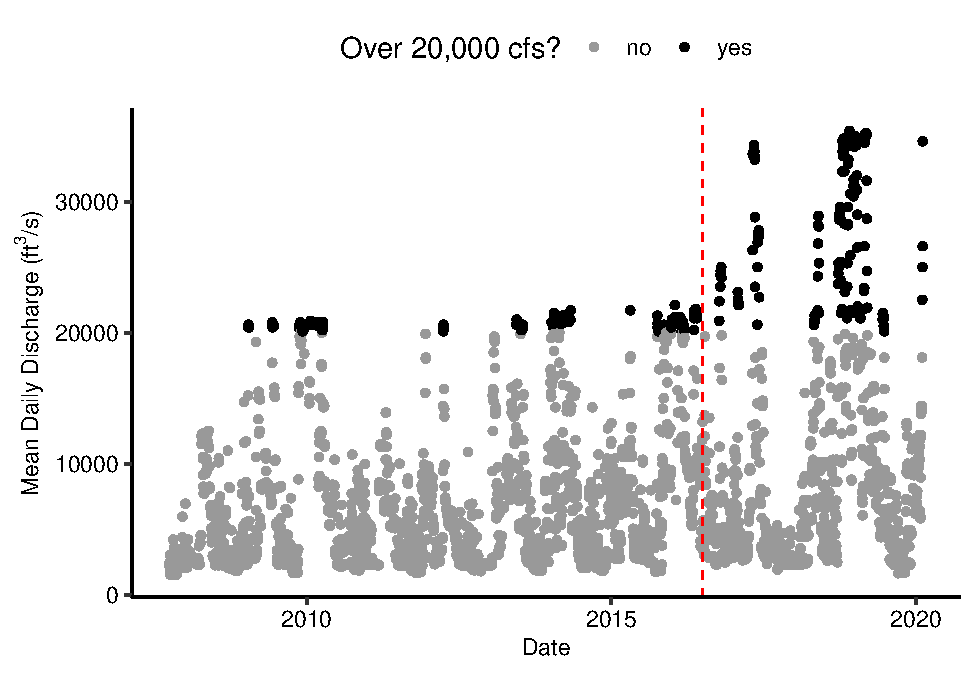
\includegraphics{Project_Template_files/figure-latex/unnamed-chunk-2-1.pdf}
\caption{Scatterplot of mean daily discharge with observations above
20,000 cubic feet per second shown in black. The red, vertical dashed
line illustrates the date the QRR was implemented.}
\end{figure}

The above plot shows an increase in observed mean daily discharges
following the QRR implementation. The number of days where mean daily
discharge exceeds 20,000 cfs increases markedly after June 2016.

\begin{longtable}[]{@{}lrrrrrr@{}}
\caption{Summary of descriptive statistics for mean daily discharge,
before and after QRR implementation.}\tabularnewline
\toprule
& Min. & 1st Qu. & Median & Mean & 3rd Qu. & Max.\tabularnewline
\midrule
\endfirsthead
\toprule
& Min. & 1st Qu. & Median & Mean & 3rd Qu. & Max.\tabularnewline
\midrule
\endhead
preQRR\_Discharge & 1510 & 2560 & 4990 & 7019 & 8715 &
22100\tabularnewline
postQRR\_Discharge & 1640 & 3000 & 5680 & 9610 & 12600 &
35400\tabularnewline
\bottomrule
\end{longtable}

Comparing the descriptive statistics for discharge before and after QRR
implementation, it can be seen that discharge is greater in the later
period for each measure of central tendency as well as the maximum and
minimum values.

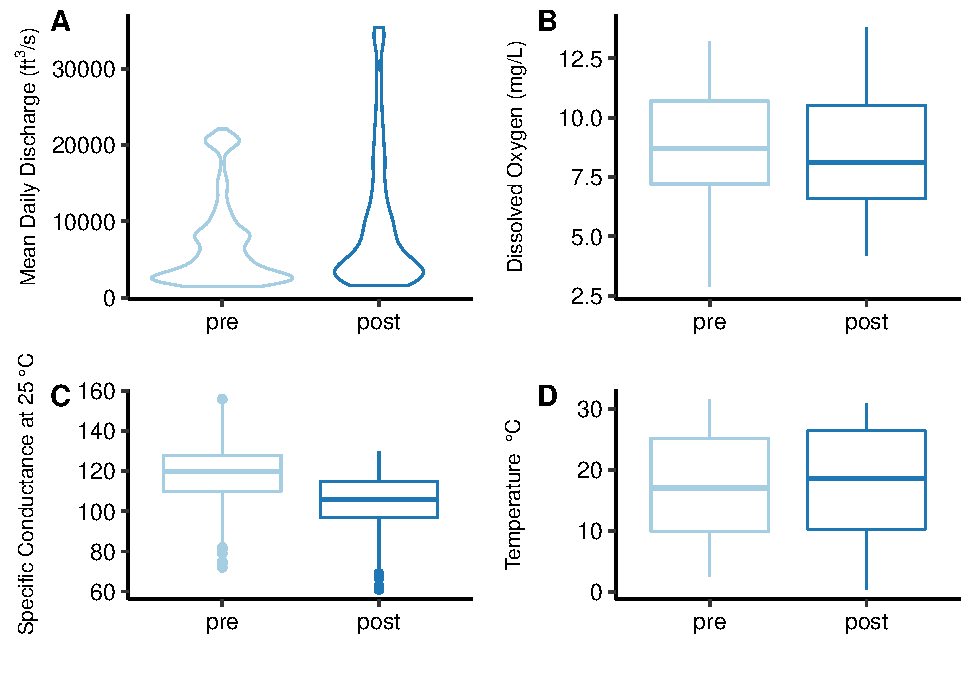
\includegraphics{Project_Template_files/figure-latex/unnamed-chunk-4-1.pdf}
In plot A, we can observe a clustering of discharge values around 20,000
cfs, which is consistent with what is known about Army Corps management
of the Kerr Dam before the QRR implementation. In comparison, the
distribution of mean daily discharge post-QRR has a longer right tail as
floodwater managers were permitted to release waters up to 35,000 cfs
for extreme wet conditions. From boxplots B and D, it is difficult to
distinguish whether dissolved oxygen readings or temperature
measurements have increased or decreased significantly. The boxplots in
plot C suggest that conductance may have decreased from the early period
to the post-QRR period.

\begin{longtable}[]{@{}lrrrrrrr@{}}
\caption{Descriptive statistics of water quality indicators pre- and
post-QRR implementation.}\tabularnewline
\toprule
& Min. & 1st Qu. & Median & Mean & 3rd Qu. & Max. & NA's\tabularnewline
\midrule
\endfirsthead
\toprule
& Min. & 1st Qu. & Median & Mean & 3rd Qu. & Max. & NA's\tabularnewline
\midrule
\endhead
preQRR\_DissolvedOxygen & 2.9 & 7.2 & 8.7 & 8.9 & 10.7 & 13.2 &
161\tabularnewline
postQRR\_DissolvedOxygen & 4.2 & 6.6 & 8.1 & 8.5 & 10.5 & 13.8 &
19\tabularnewline
preQRR\_Temperature & 2.6 & 9.9 & 17.0 & 17.4 & 25.2 & 31.6 &
24\tabularnewline
postQRR\_Temperature & 0.4 & 10.3 & 18.6 & 18.4 & 26.4 & 30.9 &
16\tabularnewline
preQRR\_Conductance & 72.0 & 110.0 & 120.0 & 118.5 & 128.0 & 156.0 &
183\tabularnewline
postQRR\_Conductance & 61.0 & 97.0 & 106.0 & 104.8 & 115.0 & 130.0 &
17\tabularnewline
\bottomrule
\end{longtable}

Between the two periods, average dissolved oxygen decreased slightly,
average temperature increased by 1 degree, and conductance decreased by
over 10\%.

\begin{figure}
\centering
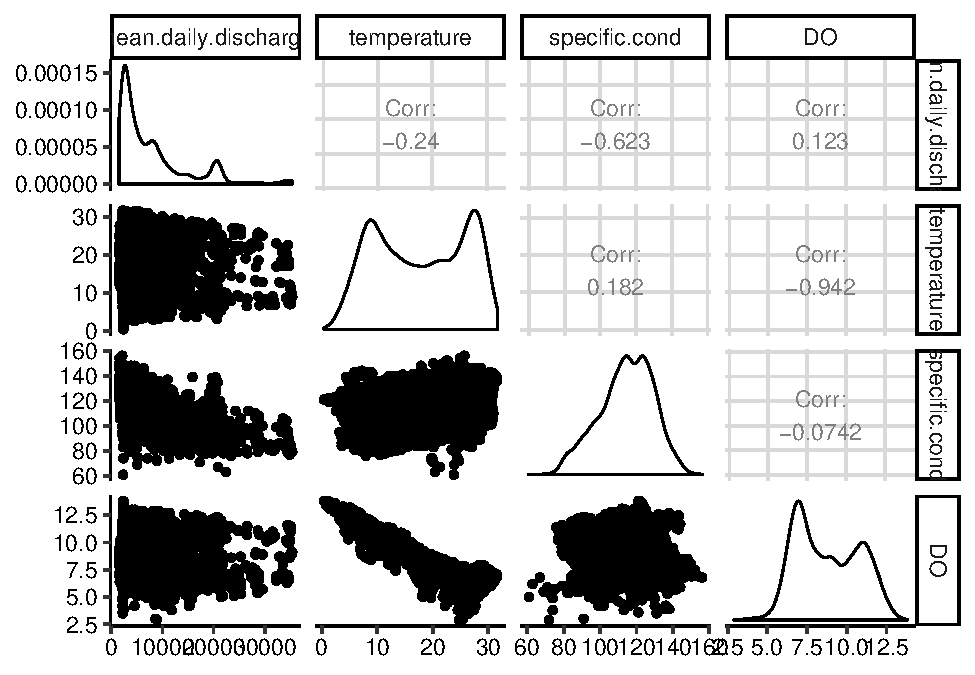
\includegraphics{Project_Template_files/figure-latex/unnamed-chunk-6-1.pdf}
\caption{Scatterplot/correlation matrix of discharge and downstream
water quality indicators.}
\end{figure}

The scatterplot matrix shows that temperature and dissolved oxygen are
highly negatively correlated (corr = -0.94), which is consistent with
the understanding that cold water can hold more dissolved oxygen. This
is important to consider for later regression analysis as there may be
an issue of endogeneity when modeling the influence of discharge on
dissolved oxygen. Specific conductance and temperature are moderately
negatively correlated (corr = 0.182). Also worth noting are the bimodal
distributions of temperature and dissolved oxygen.

\newpage

\hypertarget{analysis}{%
\section{Analysis}\label{analysis}}

\hypertarget{question-1-is-mean-daily-discharge-at-the-roanoke-rapids-gage-station-significantly-different-between-the-pre-qrr-and-post-qrr-implementation-periods}{%
\subsection{Question 1: Is mean daily discharge at the Roanoke Rapids
gage station significantly different between the pre-QRR and post-QRR
implementation
periods?}\label{question-1-is-mean-daily-discharge-at-the-roanoke-rapids-gage-station-significantly-different-between-the-pre-qrr-and-post-qrr-implementation-periods}}

\begin{figure}
\centering
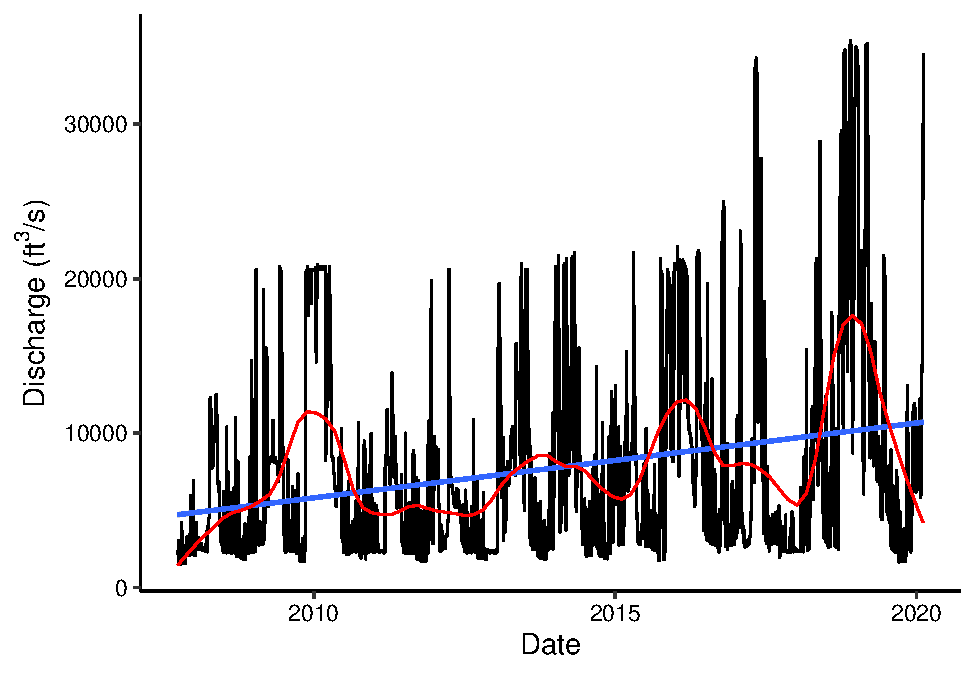
\includegraphics{Project_Template_files/figure-latex/unnamed-chunk-7-1.pdf}
\caption{Line graph of mean daily discharge over time with time series
trend (red) and line of best fit for original data (blue).}
\end{figure}

The above line graph shows a red trend line from the decomposed time
series of mean daily discharge at the Roanoke Rapids gage station. The
blue line of best fit for the discharge data illustrates a positive
trend in mean daily discharge.

Given that mean daily discharges before and after implementation of the
QRR were not normally distributed and did not exhibit equal variance, a
non-parametric one-way ANOVA was used to compare the two groups. The
results indicated that mean daily discharge after implementation of the
QRR is statistically different from mean daily discharge before QRR
implementation (Kruskal-Wallis; df = 1; chi-squared = 71.7; p-value
\textless{} 0.0001).

In light of this finding and the preliminary exploration of the mean
daily discharge distributions, it can be concluded that mean daily
discharge after the implementation of the QRR regime is significantly
greater than mean daily discharge before its implementation.

\hypertarget{question-2-how-does-discharge-relate-to-downstream-water-quality-indicators}{%
\subsection{Question 2: How does discharge relate to downstream water
quality
indicators?}\label{question-2-how-does-discharge-relate-to-downstream-water-quality-indicators}}

\begin{figure}
\centering
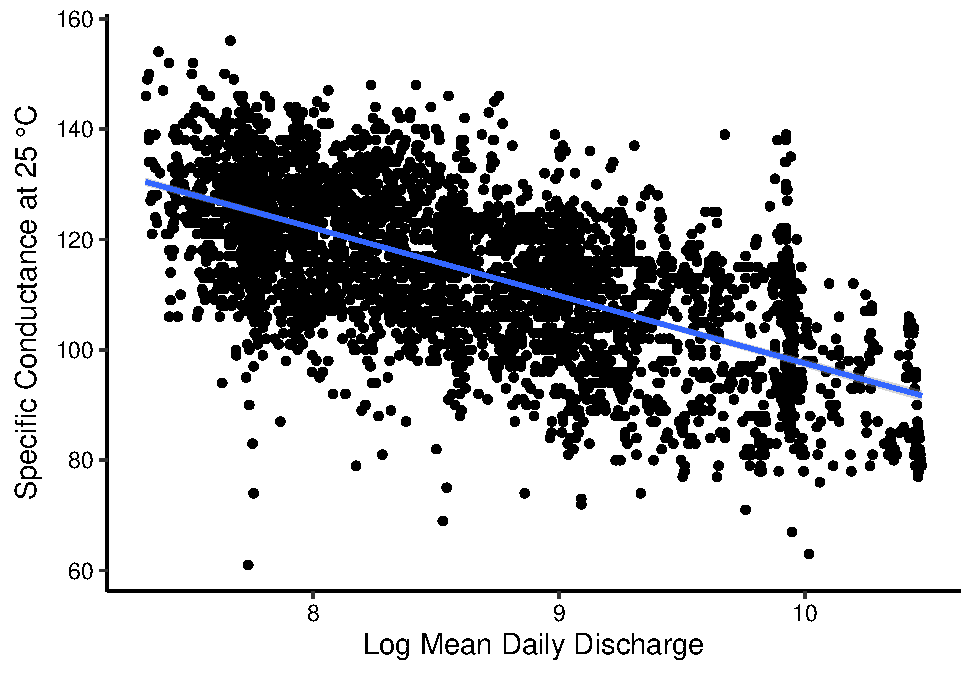
\includegraphics{Project_Template_files/figure-latex/unnamed-chunk-10-1.pdf}
\caption{Regression of specific conductance on log mean daily
discharge.}
\end{figure}

A log transformation of mean daily discharge resulted in a better model
fit when regressing specific conductance on discharge (R2 = 0.43 vs.~R2
= 0.39). Based on the regression results, there is a significant
negative relationship between mean daily discharge and specific
conductance at 25 degrees celsius, and mean daily discharge accounts for
about 43\% of the total variance in specific conductance (simple linear
regression; R2 = 0.43; df = 4315; p-value \textless{} .0001).
Furthermore, a 1\% increase in mean daily discharge is associated with a
decrease in specific conductance of about 0.12 uS/cm.

\newpage

\begin{figure}
\centering
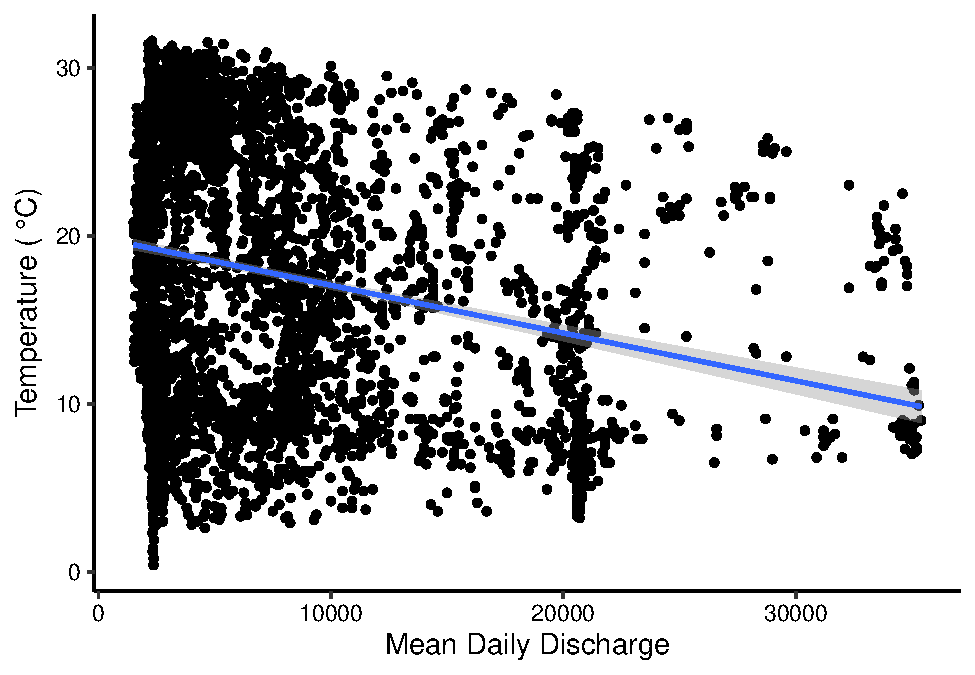
\includegraphics{Project_Template_files/figure-latex/unnamed-chunk-12-1.pdf}
\caption{Regression of temperature on mean daily discharge.}
\end{figure}

Based on the results of regressing temperature on mean daily discharge,
there is a statistically significant, but very weak negative
relationship between mean daily discharge and temperature (simple linear
regression; R2 = 0.06; df = 4475; p-value \textless{} .0001). A one
cubic foot per second increase in mean daily discharge is associated
with a 0.0002 degree Celsius decrease in temperature. The model accounts
for only 6\% of the total variance in temperature.

\newpage

\begin{figure}
\centering
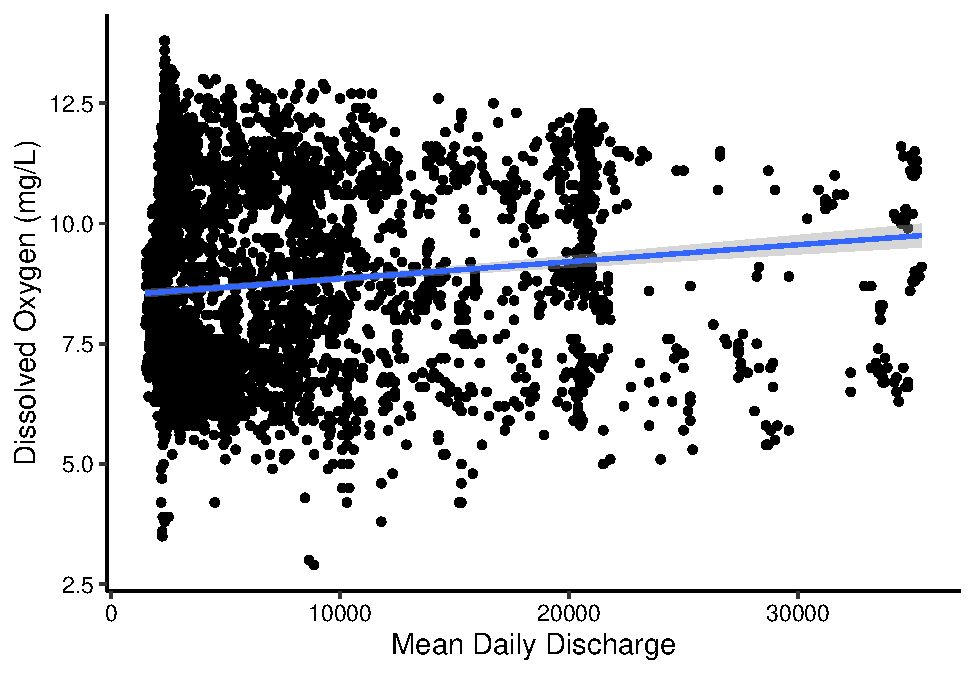
\includegraphics{Project_Template_files/figure-latex/unnamed-chunk-14-1.pdf}
\caption{Regression of dissolved oxygen on mean daily discharge with no
interaction effect.}
\end{figure}

Due the high degree of correlation between temperature and dissolved
oxygen, an interaction effect between temperature and discharge was
incorporated into the regression analysis for dissolved oxygen. Whereas
the first model (without an interaction effect; pictured above)
indicated a statistically significant relationship between discharge and
dissolved oxygen, the improved model showed no significant relationship
between the two variables (simple linear regression; R2 = 0.90; df =
4333; p-value \textless{} .0001). The coefficient for mean daily
discharge was very close to zero with a statistically insignificant
p-value. However, due to the inclusion of temperature as a predictor,
the model still predicted around 90\% of the total variance in dissolved
oxygen.

\newpage

\hypertarget{summary-and-conclusions}{%
\section{Summary and Conclusions}\label{summary-and-conclusions}}

Based on the results of a non-parametric one-way ANOVA test, there is
strong evidence to suggest that average daily discharges at the Roanoke
Rapids gage station increased with the introduction of the
quasi-run-of-the-river floodwater management regime. This result may be
unsurprising given that the QRR regime increases the maximum level of
discharges that managers are permitted to release during extreme wet
conditions. However, we might also expect that the management regime
would not change the volume of water that must be released each year, so
the findings are interesting in that respect.

As for the second research question, the results suggested that
discharge may be a good predictor of specific conductance. Based on the
regression model, discharge could be used to predict about 43\% of the
total variation in conductance. However, this level of analysis is not
sufficient to determine whether there is a causal relationship between
discharge and conductance.

The results of the temperature regression model provide only weak
evidence of a relationship between discharge and temperature. Although
the discharge coefficient was statistically significant, its magnitude
near zero does not suggest a strong relationship between the two
variables. There may be confounding factors, like weather patterns, for
example, that influence both temperature and discharge.

Finally, based on the analysis, there is no evidence to suggest that
discharge is a good predictor of dissolved oxygen. Whereas preliminary
modeling suggested a significant, albeit weak, relationship between
discharge and dissolved oxygen, there was no significant relationship
present after accounting for the effect of temperature on dissolved
oxygen.

The analysis would be made more robust by including additional variables
that might explain variation in water quality indicators. Factors like
weather or climate, land use along the Roanoke, and biological factors
were not included in this analysis but are likely to impact water
temperature, dissolved oxygen, and specific conductance. If those
factors were built into a random effects model along with discharge as
an independent variable, we might get a better sense of the true
influence of discharge on those indicators.

Another strategy to consider would be to introduce lag into the models,
since it may take time for changes in discharge to effect indicators
downstream. Removing the seasonality in the data might also provide a
clearer view of the effect of discharge on water quality indicators.

\newpage

\hypertarget{references}{%
\section{References}\label{references}}

Opperman, J., Lakly, M., Peoples, C., Gastelumendi , J., \& Paiz, M.-C.
(2017, December 1). Knowledge is Power - Hydro Review. Retrieved from
\url{https://www.hydroreview.com/2017/12/01/knowledge-is-power/}

Rose, D. (2016, June 8). Army Corp approves QRR. Retrieved from
\url{http://www.lakegastongazette-observer.com/news/article_252eafe2-2d87-11e6-b575-6f234f7cf0ee.html}

\end{document}
